\chapter{Prologue}
This course was originally developed by Dr Wayne Stewart (formerly of The
University of
Auckland) and was first offered in 2009 (Figure~\ref{fig:wayne}).
I joined the Department of Statistics in July 2012
and took over the course from him. It was good fortune for me that Wayne left
the university as I arrived: if I had been able to choose which undergraduate
course I would most like to teach, it would have been this one!

Wayne is a passionate Bayesian\footnote{Bayesian statistics has a way of
creating extreme enthusiasm among its users. I don't just {\it use} Bayesian
methods, I {\it am a Bayesian}.}
and advocate
for the inclusion of Bayesian statistics in the undergraduate
statistics curriculum. I also consider myself a Bayesian and agree that this
approach to statistics should form a greater part of a statistics education
than it does today. 
While this edition of the course differs from Wayne's in some ways\footnote{
The differences are mostly cosmetic. 90\% of the content is the same.},
I hope I am able to do the topic justice in an accessible way.

\begin{figure}
\begin{center}
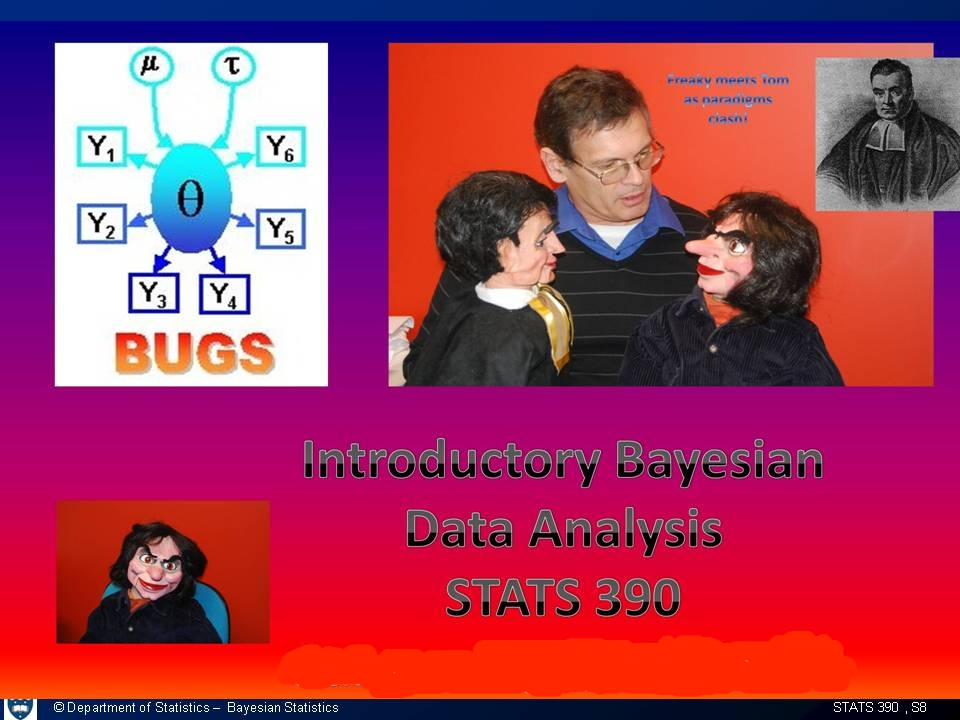
\includegraphics[scale=0.5]{Figures/390course.jpg}
\end{center}
\caption{An ad for the original version of this course (then called
STATS 390), showing Wayne Stewart with two ventriloquist dolls, who would
have debates about statistics.\label{fig:wayne}}
\end{figure}

In this course we will use the following software:
\begin{itemize}
\item R ({\tt http://www.r-project.org/})
\item JAGS ({\tt http://mcmc-jags.sourceforge.net/})
\item The {\tt rjags} package in R
\item RStudio ({\tt http://www.rstudio.com/})
\end{itemize}
You will probably have used R, at least a little bit, in previous statistics
courses. RStudio is just a nice program used for editing R code, and if you
don't like it, you're welcome to use any other text editor. JAGS is in a
different category: you most likely won't have seen it before. JAGS is used to
implement Bayesian methods in a straightforward way, and {\tt rjags} allows us
to use JAGS from within R.
Don't worry, it's not too difficult to learn and use JAGS! We will have a lot of
practice using it in the labs.

These programs are all free and open source software.
That is, they are free to use, share and modify. They should work on
virtually any operating system including the three most popular:
Microsoft Windows, Mac OS X and GNU/Linux. In previous editions of the course,
WinBUGS was used instead of JAGS. However, WinBUGS has not been updated for
several years, and only works on Microsoft Windows. The differences between
the two are fairly minor, but JAGS has the advantage of being open source and
cross-platform. All of this software is already installed on the lab computers,
but if you would like to install it on your own computer, instructions are
provided on the Course Information Sheet.

\section{Bayesian and Classical Statistics}
Throughout this course we will see many examples of Bayesian analysis, and we
will sometimes mention or compare our results with what you get from
{\it classical} or {\it frequentist} statistics, which is the other way of
doing things. You will have seen some classical statistics methods in STATS
10X and 20X (or BioSci 209), and possibly other courses as well.
You may have also seen and used Bayes' rule before (Bayes' rule can sometimes
be used in classical stats, but in Bayesian stats it is used
{\it all the time}).

Many
people have differing views on the status of these two ways of doing statistics.
In the past, Bayesian statistics was controversial, and you had to be very
brave to admit to using it! Many people were {\bf anti}-Bayesian.
Those people are now
rare: instead of Bayesians and anti-Bayesians, it would be more realistic to
say there are now Bayesians and non-Bayesians, and many of the non-Bayesians
would be happy to use Bayesian statistics in some circumstances.
The non-Bayesians would say that
Bayesian statistics is {\it one way} of doing things, and it is a matter of
choice which way you prefer to use. In my opinion, Bayesian
statistics is {\it the right way} to do things, and non-Bayesian methods are
best thought of as either approximations (sometimes very good ones!)
or alternative methods that are only to be used when the Bayesian solution
would be too hard to calculate.

Sometimes I may give strongly worded opinions on this issue, but
there is one point that you should keep in mind throughout
this course, and it is very important:

\begin{center}
\begin{tabular}{|c|}
\hline
{\bf You do not have to agree with me in order to do well in STATS 331!}\\
\hline
\end{tabular}
\end{center}

\section{This Version of the Notes}
Wayne Stewart taught STATS 331 with his own course notes. When I took over the
course, I found that our styles were fairly different, even though were teaching
the same ideas. Unfortunately, it was challenging for the students to reconcile
my explanations with Wayne's. Therefore I thought it would be better to have
my own version of the notes. Since 2013 is the first year with this version, you
should not expect them to be complete: there are many things that are important
and examinable, that will be only discussed in lectures, labs and assignments!

The plots in these notes were not produced using R, but using a different
plotting package where I am more familiar with the advanced plotting features.
This means that when I give an R command for a plot,
it will not produce a plot that looks {\it exactly} like the plot that follows.
However, it will give approximately the same plot, conveying the same information.
I apologise if you find this inconsistency distracting.

At this stage, the course notes contain the basic material of the course. Some
more advanced topics will be introduced and discussed in lectures, labs and
assignments.

\begin{framed}
\begin{center}
{\bf 
I appreciate any feedback you may have about these notes.
}
\end{center}
\end{framed}

\section{Assessment}
The assessment for this course is broken down as follows:
\begin{itemize}
\item 20\% Assignments. There will be four assignments, worth 5\% each. The
assignments are not small, so please do not leave them until the last minute.
\item 20\% Midterm test (50 minutes, calculators permitted). This will be held
in class, in place of a lecture, some time just after mid semester break.
\item 60\% Final exam (two hours, calculators permitted).
\end{itemize}

